% Computational Sections for "Computational Modelling of Bipolar Disorder"
% Draft technical contribution — Mahault Albarracin
% Sections 3–7: Model, Affective Readout, Simulation, Results, Discussion

\section{Generative Model}\label{sec:model}

We formalise counterfactual temporal framing as policy selection within a partially observable Markov decision process (POMDP), following the active inference framework \citep{parr2022active}. The agent maintains beliefs over a factored hidden state space and selects among temporally oriented policies that differentially redistribute precision across state transitions.

\subsection{Factored State Space}

The hidden state $s = (v, e, f)$ is factored into three dimensions:

\begin{itemize}
    \item \textbf{Valence} $v \in \{0, \ldots, K{-}1\}$: The agent's affective state, discretised at granularity $K$. This is the key parameter corresponding to the \emph{granularity of the higher-order state space} described in the abstract. At $K{=}4$, the agent has a coarse attractor landscape with few intermediate states; at $K{=}8$, intermediate states (e.g., irritation, mild contentment) become representable.

    \item \textbf{Energy} $e \in \{0, \ldots, M{-}1\}$: An interoceptive resource estimate ($M{=}8$), modelling the metabolic or energetic budget available for action. This hidden state enables the switching dynamical system structure underlying bipolar oscillation: manic episodes deplete the energy budget through aggressive future-oriented framing, while a homeostatic recovery mechanism prevents permanent collapse and enables cycling.

    \item \textbf{Temporal frame} $f \in \{\textsc{past}, \textsc{present}, \textsc{future}\}$: The currently active counterfactual orientation. \textsc{past} corresponds to backward-facing precision modulation (autobiographical counterfactual simulation); \textsc{present} to standard perception--action coupling; \textsc{future} to forward-facing precision modulation (prospective counterfactual simulation toward a ``solution state'').
\end{itemize}

The total state space has dimensionality $K \times M \times 3$. Under the factored representation, transition and observation matrices decompose into factor-specific components, yielding a compact specification.

\subsection{Observation Model}

The agent receives three observation modalities, each generated by a likelihood mapping $\mathbf{A}_m$:

\begin{enumerate}
    \item \textbf{Environmental feedback} $o_{\text{ext}} \in \{\text{negative}, \text{neutral}, \text{positive}\}$: Depends on both valence and energy. Higher valence and energy increase the probability of positive feedback, modelling the bidirectional relationship between affective state and environmental engagement.

    \item \textbf{Interoceptive signal} $o_{\text{int}} \in \{\text{depleted}, \text{neutral}, \text{energised}\}$: Depends on the true energy state, with precision controlled by the parameter $\omega_e$. When $\omega_e$ is high, the agent accurately reads its metabolic state; when low, the interoceptive signal is blurred, and the agent cannot distinguish depletion from energy availability.

    \item \textbf{Felt valence} $o_{\text{val}} \in \{0, \ldots, K{-}1\}$: A mapping from the valence state whose precision scales with granularity $K$. At high $K$, the agent can make fine-grained distinctions among affective states; at low $K$, self-observation is blurred, and the negative prior has lasting influence over beliefs.
\end{enumerate}

Critically, the \emph{agent's generative model} of $\mathbf{A}_{\text{int}}$ may differ from the environment's true observation-generating process. This mismatch---the agent's interoceptive model being less precise than reality---is the computational mechanism underlying mania: the environment provides accurate energy depletion signals, but the agent's blurred $\mathbf{A}_{\text{int}}$ prevents these signals from updating beliefs about resource availability.

\subsection{Transition Model: Temporal Framing as Policy}

Each action (temporal framing mode) defines a distinct transition structure $\mathbf{B}_a = \mathbf{B}_v^{(a)} \otimes \mathbf{B}_e^{(a)} \otimes \mathbf{B}_f^{(a)}$, where $\otimes$ denotes the Kronecker product over factored transition matrices.

\paragraph{RECALL (past-oriented framing).}
The valence transition $\mathbf{B}_v^{\textsc{recall}}$ pulls the affective state toward the prior $\mathbf{D}$---specifically, toward positively valenced states. The strength of this pull is controlled by $\pi_{\text{pos}}$ through a sigmoidal gating function $\alpha = \sigma(\pi_{\text{pos}} - \theta)$. When $\pi_{\text{pos}}$ is high, RECALL effectively generates positive counterfactuals grounded in a confident self-model; when $\pi_{\text{pos}}$ is low, the pull is negligible, and past-oriented counterfactuals fail to sustain positive affect. Crucially, this impairment is not merely a matter of belief: in the generative process, recall effectiveness is gated by the same biological parameter, modelling the finding that depressed individuals show impaired access to specific positive autobiographical memories \citep{williams2007autobiographical}. Energy cost is minimal.

\paragraph{ENGAGE (present-oriented framing).}
Standard perception--action coupling. Valence evolves as a random walk centred on the current state, driven primarily by environmental feedback. Energy is sustainable---ENGAGE does not deplete the metabolic budget, though a background metabolic cost applies to all active states.

\paragraph{FUTURATE (future-oriented framing).}
The valence transition pulls toward the most positive state---the ``solution state''---modelling the generation of a highly precise prospective counterfactual. The effectiveness of this pull in the generative process is modulated by reward sensitivity ($c_{\text{scale}}$): an anhedonic agent cannot generate positive future affect even when imagining optimistic scenarios. Energy cost is high, reflecting the intensive environmental sampling and goal-directed behaviour associated with future-oriented framing. The frame transition is strongly absorbing: once in \textsc{future} mode, the agent tends to remain there.

\paragraph{REST (conservation).}
Valence drifts toward neutral, energy recovers rapidly, and the frame opens to any orientation. This models the conservation prior that activates when resource depletion is detected.

\subsection{Preferences and Prior}

The preference vectors $\mathbf{C}_m$ encode the agent's prior expectations about desirable observations: positive environmental feedback, feeling energised, and positive valence. These preferences are scaled by the reward sensitivity parameter $c_{\text{scale}}$, which modulates the \emph{precision} of hedonic predictions. When $c_{\text{scale}}$ is low, the agent is anhedonic: it does not strongly distinguish between positive and negative outcomes, leading to flattened motivation and near-random policy selection. When $c_{\text{scale}}$ is high, the agent is reward-hypersensitive, aggressively pursuing positive outcomes at the expense of energy conservation.

The prior $\mathbf{D}$ over initial states is shaped by $\pi_{\text{pos}}$: higher $\pi_{\text{pos}}$ concentrates mass on positive valence states, reflecting a confident, positively biased self-model. This prior serves a dual role---it initialises beliefs \emph{and} provides the attractor for RECALL transitions.

\subsection{Clinical Parameters}

Four parameters capture the computational dimensions of vulnerability:

\begin{table}[h]
\centering
\begin{tabular}{llll}
\toprule
\textbf{Parameter} & \textbf{Role} & \textbf{Low value} & \textbf{High value} \\
\midrule
$\pi_{\text{pos}}$ & Positive-belief precision & Cannot generate positive past counterfactuals & Stable narrative sustains affect \\
$K$ & Affective granularity & Coarse attractors; catastrophic transitions & Fine-grained; smooth regulation \\
$\omega_e$ & Interoceptive precision & Cannot detect depletion (mania risk) & Accurate metabolic monitoring \\
$c_{\text{scale}}$ & Reward sensitivity & Anhedonia; flattened hedonic response & Hypersensitivity; exaggerated pursuit \\
\bottomrule
\end{tabular}
\caption{Clinical parameters and their computational roles.}
\label{tab:params}
\end{table}

The first three parameters are orthogonal: they affect distinct components of the generative model ($\mathbf{D}$ prior and $\mathbf{B}$ matrices, state space dimensionality, and $\mathbf{A}$ matrix precision, respectively). The fourth parameter ($c_{\text{scale}}$) modulates the $\mathbf{C}$ vectors that drive policy selection via expected free energy, and also gates action effectiveness in the generative process---capturing the biological reality that anhedonia impairs both the motivation to act and the hedonic impact of action outcomes.


\section{Affective Readout}\label{sec:affect}

Following \citet{pattisapu2024free}, we derive both valence and arousal from the agent's free energy, grounding the simulation in a circumplex model of emotion.

\subsection{Valence}

Valence is computed as a reward prediction error---the difference between the utility of the actual observation and its expected value under the agent's predictive model:
\begin{equation}
    V = U - \mathbb{E}[U]
\end{equation}
where $U = \sum_m \log P(o_m \mid C_m)$ is the utility of the observed outcome given preferences, and $\mathbb{E}[U] = \sum_m \sum_{o} Q(o_m \mid \pi) \log P(o_m \mid C_m)$ is the expected utility under predicted observations $Q(o_m \mid \pi) = \mathbf{A}_m \, q_{\text{pred}}$. Positive valence signals a ``better than expected'' outcome; negative valence signals worse than expected.

\subsection{Arousal}

Arousal is the entropy of the posterior belief distribution:
\begin{equation}
    A = H[Q(s \mid o)] = -\sum_s Q(s \mid o) \log Q(s \mid o)
\end{equation}
normalised by maximum entropy $\log |\mathcal{S}|$ to yield $A_{\text{norm}} \in [0, 1]$. High arousal reflects posterior uncertainty---the agent does not know what state it is in---and is functionally linked to the amygdala's role as a learning signal for allostatic regulation \citep{barrett2017theory}.

\subsection{Circumplex Transformation}

To map the agent's trajectory onto the circumplex model, we centre arousal as $A_c = 2 A_{\text{norm}} - 1 \in [-1, 1]$, so that low posterior entropy (certainty) corresponds to calm ($A_c < 0$) and high entropy (uncertainty) corresponds to alertness ($A_c > 0$). The polar transformation
\begin{equation}
    r = \sqrt{V^2 + A_c^2}, \qquad \theta = \arctan(A_c / V)
\end{equation}
then places the agent's emotional state within the standard circumplex \citep{russell1980circumplex}, with $0^\circ$ = Happy, $90^\circ$ = Alert, $180^\circ$ = Sad, $270^\circ$ = Calm.

\subsection{Temporal Derivatives (Joffily \& Coricelli)}

In parallel, we track the variational free energy $F(t)$ at each timestep and compute:
\begin{itemize}
    \item \textbf{Valence (J-C)}: $\tanh(-\Delta F / \tau)$, capturing the \emph{rate} of free energy change
    \item \textbf{Anticipation}: $-\Delta^2 F$, capturing curvature---positive for hope, negative for fear
\end{itemize}
This dual readout allows us to examine both the \emph{momentary} affective state (Pattisapu: how does the current observation compare to expectation?) and the \emph{trajectory} of affective dynamics (Joffily-Coricelli: is free energy increasing or decreasing over time?).


\section{Simulation Design}\label{sec:simulation}

\subsection{Clinical Profiles}

We define three parameter configurations corresponding to the phenotypes described in the abstract:

\paragraph{Healthy.} $\pi_{\text{pos}} = 5.0$, $K = 8$, $\omega_e = 5.0$, $c_{\text{scale}} = 1.0$. High-precision positive self-beliefs enable effective RECALL. Fine-grained affective state space permits smooth regulation. Accurate interoception supports adaptive energy management. Normal reward sensitivity drives appropriately motivated policy selection.

\paragraph{Depressive.} $\pi_{\text{pos}} = 0.2$, $K = 4$, $\omega_e = 5.0$, $c_{\text{scale}} = 0.1$. Very low precision on positive beliefs renders RECALL biologically ineffective---past-oriented counterfactuals fail to access or sustain positive affect. Reduced affective granularity ($K{=}4$) limits the resolution of affective self-monitoring. Interoception remains accurate; the agent \emph{can} detect its state but \emph{cannot} change it through narrative. Critically, reward sensitivity is severely attenuated ($c_{\text{scale}} = 0.1$), modelling anhedonia: the agent does not strongly distinguish between positive and negative outcomes, leading to near-random policy selection and an inability to generate positive affect even through future-oriented imagination.

\paragraph{Manic.} $\pi_{\text{pos}} = 5.0$, $K = 4$, $\omega_e = 0.5$, $c_{\text{scale}} = 2.0$. Strong positive beliefs and \emph{hypersensitive} reward processing ($c_{\text{scale}} = 2.0$) drive aggressive pursuit of positive outcomes through both RECALL and FUTURATE. The elevated $\mathbf{C}$-vector precision amplifies the expected free energy difference between positive and negative outcomes, biasing the agent toward high-valence policies regardless of their energy cost. Low interoceptive precision ($\omega_e = 0.5$) prevents the agent from detecting the resulting energy depletion.

\subsection{Experimental Protocol}

Each profile is run for $T = 300$ timesteps in a stochastic environment with volatility $p = 0.45$ (probability of random valence perturbation per step, with a mild negative bias). The environment modulates action effectiveness through the clinical parameters: recall effectiveness is gated by $\sigma(\pi_{\text{pos}} - \theta)$, and futurate effectiveness is gated by $c_{\text{scale}}$. This captures the biological reality that these parameters affect not only the agent's \emph{beliefs} about what actions will achieve, but also what they \emph{actually} achieve.

The environment includes three additional mechanisms:
\begin{itemize}
    \item \textbf{Homeostatic energy recovery}: When energy falls below a baseline ($M/3$), a natural recovery drift prevents permanent depletion.
    \item \textbf{Bidirectional valence--energy coupling}: Low energy probabilistically reduces valence (crash), while persistently low valence drains energy (motivational fatigue / anhedonia).
    \item \textbf{Background metabolic cost}: All non-REST actions have a small probability of energy depletion, ensuring that sustained activity requires periodic recovery.
\end{itemize}

\subsection{Granularity Sweep}

To isolate the effect of affective granularity, we fix $\pi_{\text{pos}} = 3.0$, $\omega_e = 0.8$, and $c_{\text{scale}} = 1.0$ and sweep $K \in \{2, 4, 6, 8\}$ across 5 independent runs per value. We measure: (a) valence variance (oscillation amplitude), (b) jump-size distribution $|\Delta v_t|$, (c) action selection proportions.

\subsection{Parameter Landscape}

We sweep $\pi_{\text{pos}} \in [0.1, 8.0]$ and $\omega_e \in [0.1, 8.0]$ over a $10 \times 10$ grid (fixing $K{=}4$, $M{=}8$, $c_{\text{scale}} = 1.0$, $T{=}200$) and compute mean believed valence, valence variance, mean believed energy, and action entropy.


\section{Results}\label{sec:results}

\subsection{Phenotype Differentiation}

The three clinical profiles produce qualitatively distinct trajectories (Figure~\ref{fig:phenotypes}).

The \textbf{healthy} agent maintains moderate-high mean valence ($\bar{v} = 0.62$) and near-maximal energy ($\bar{e} = 0.97$). Policy selection shows a clear structure: RECALL dominates, supplemented by ENGAGE and periodic REST episodes for energy management. The Joffily-Coricelli valence signal oscillates symmetrically around zero, indicating balanced prediction error dynamics (Figure~\ref{fig:joffily}, left).

The \textbf{depressive} agent exhibits persistently low valence ($\bar{v} = 0.54$) and moderate energy depletion ($\bar{e} = 0.76$). Policy selection is near-uniform across actions---a direct consequence of anhedonia ($c_{\text{scale}} = 0.1$) flattening the preference vectors and rendering all actions similarly valued under expected free energy. Combined with biologically impaired recall effectiveness ($\sigma(\pi_{\text{pos}} - \theta) \approx 0.12$) and attenuated futurate effectiveness ($c_{\text{scale}} = 0.1$), the few recall and futurate attempts that occur have only a 10--12\% chance of improving valence. The result is the pattern described in the abstract: ``uncertainty remains diffusely distributed across temporal horizons.'' The energy depletion reflects a secondary mechanism: persistently low valence triggers motivational fatigue (the bidirectional valence--energy coupling).

The \textbf{manic} agent shows the highest mean valence ($\bar{v} = 0.72$) but the lowest energy ($\bar{e} = 0.66$)---the characteristic manic dissociation between subjective well-being and objective resource depletion. Hypersensitive reward processing ($c_{\text{scale}} = 2.0$) drives aggressive selection of RECALL and FUTURATE, both effective for valence but energetically costly. The energy trace shows periods of depletion followed by partial recovery, producing the oscillatory pattern characteristic of bipolar cycling. The Joffily-Coricelli $F(t)$ trace is notably flat (Figure~\ref{fig:joffily}, right), reflecting that the manic agent's overconfident model is largely impervious to prediction errors.

\subsection{Granularity and Oscillation Dynamics}

The granularity sweep (Figure~\ref{fig:granularity}) provides direct computational evidence for the abstract's claim that ``reduced granularity in higher-order belief distributions constrains the generation of future-oriented counterfactuals for resolving uncertainty.''

Valence variance decreases with granularity: $0.10$ at $K{=}2$, $0.039$ at $K{=}4$, $0.035$ at $K{=}6$, and $0.037$ at $K{=}8$---a near three-fold reduction from the coarsest to the finest resolution, with diminishing returns above $K{=}4$. The jump-size distribution is heavy-tailed at $K{=}2$ (catastrophic transitions), whereas for $K \geq 4$ it concentrates near zero.

This result formalises the clinical observation that emotional granularity is a protective factor against mood instability \citep{barrett2017theory}. In our model, the protection is mechanistic: higher $K$ increases the resolution of both the $\mathbf{B}_v$ matrix and the $\mathbf{A}_{\text{val}}$ observation model, enabling smaller steps through the affective landscape rather than all-or-nothing transitions.

\subsection{Circumplex Emotional Trajectories}

Mapping valence and arousal onto the circumplex (Figure~\ref{fig:circumplex}) reveals distinct emotional signatures.

The \textbf{healthy} agent's trajectory occupies a compact region near the Happy--Excited boundary (positive valence, moderate arousal), consistent with adaptive exploration.

The \textbf{depressive} agent shows the widest spread across the circumplex, reaching into the Alert--Angry and Sad--Depressed quadrants. This dispersed trajectory reflects emotional instability driven by near-random policy selection, consistent with clinical findings of affect instability in depression \citep{houben2015relation}.

The \textbf{manic} agent clusters tightly near Excited/Happy, reflecting elevated but narrowly distributed positive affect that masks deteriorating metabolic resources.

\subsection{Parameter Landscape}

The parameter sweep (Figure~\ref{fig:landscape}) reveals a clinical landscape with identifiable regions:

\begin{itemize}
    \item \textbf{Low $\omega_e$, moderate-high $\pi_{\text{pos}}$}: Lower mean valence, elevated variance, depleted energy. The manic-vulnerable zone.
    \item \textbf{Low $\pi_{\text{pos}}$, high $\omega_e$}: Moderate-low valence with low action entropy. The depressive zone---the agent can track its state but cannot generate positive counterfactuals.
    \item \textbf{High $\pi_{\text{pos}}$, high $\omega_e$}: Highest valence, stable energy, moderate action entropy. The healthy zone.
\end{itemize}


\section{Discussion}\label{sec:discussion}

\subsection{Narrative Regulation as Policy Selection}

The model formalises the paper's central claim---that ``strategic narratives are dynamically self-maintaining structures''---by casting temporal framing as active inference policy selection. RECALL, ENGAGE, FUTURATE, and REST are not merely cognitive strategies; they are policies with distinct transition dynamics that the agent selects by minimising expected free energy.

The depressive phenotype illustrates narrative failure through multiple reinforcing mechanisms: RECALL cannot sustain positive affect (low $\pi_{\text{pos}}$ impairs both the belief about and the biological effectiveness of positive memory access), FUTURATE cannot generate positive affect (anhedonia blocks the hedonic impact of prospective simulation), and the resulting near-random policy fails to counteract the negative environmental drift. The manic phenotype illustrates narrative disconnection from metabolic evidence: FUTURATE successfully generates positive affect and is aggressively pursued due to reward hypersensitivity, but at an energetic cost invisible to the agent's blurred interoceptive model.

\subsection{Anhedonia as Flattened Preference Precision}

The introduction of reward sensitivity ($c_{\text{scale}}$) captures a dimension of depression distinct from both cognitive pessimism ($\pi_{\text{pos}}$) and emotional granularity ($K$). Anhedonia is modelled as reduced precision on the preference vectors $\mathbf{C}$, which flattens the expected free energy landscape and makes all policies appear approximately equivalent. The depressive agent does not actively choose to withdraw; it simply cannot distinguish between action outcomes. This is consistent with reinforcement learning accounts of anhedonia as impaired reward prediction \citep{huys2013mapping} and with the clinical presentation of motivational deficit rather than active avoidance.

Conversely, the manic agent's elevated $c_{\text{scale}}$ corresponds to reward hypersensitivity---the amplified hedonic response to positive outcomes that drives excessive goal pursuit.

\subsection{Granularity as a Transdiagnostic Vulnerability}

The granularity parameter $K$ captures a vulnerability dimension orthogonal to both positive-belief precision and interoceptive accuracy. Low $K$ is not a mood state but a structural property of the generative model---it constrains the \emph{resolution} at which affect can be represented. Importantly, $K$ also determines the precision of $\mathbf{A}_{\text{val}}$: lower granularity means blurred self-observation of affect, so that negative priors persist longer.

This has direct implications for intervention. Increasing emotional granularity (through psychoeducation, mindfulness, or affect labelling) changes the \emph{dimensionality of the space} in which affective regulation occurs and the \emph{precision} of affective self-monitoring. Our simulation shows that this alone reduces oscillation amplitude approximately three-fold.

\subsection{The Energy Budget and Bipolar Oscillation}

The inclusion of energy as a latent state enables bipolar cycling to emerge from precision dynamics without hard-coding mood states. The oscillation follows a natural cycle: (1) reward hypersensitivity drives FUTURATE selection; (2) FUTURATE depletes energy; (3) blurred interoception prevents detection of depletion; (4) environmental feedback eventually overwhelms the optimistic model; (5) the agent transitions to REST; (6) homeostatic recovery restores energy; (7) the cycle repeats.

This switching dynamical system structure---driven by the interaction between miscalibrated interoceptive precision ($\omega_e$) and amplified reward sensitivity ($c_{\text{scale}}$)---resonates with clinical accounts of bipolar disorder as a disorder of energy regulation \citep{berk2007stages}. The model predicts that interventions targeting interoceptive accuracy would reduce oscillation amplitude independently of interventions targeting narrative capacity or emotional granularity.

\subsection{Two Formulations of Valence}

The dual affective readout---\citeauthor{pattisapu2024free}'s reward prediction error alongside \citeauthor{joffily2013emotional}'s temporal derivative---reveals complementary aspects of affective dynamics. The Pattisapu formulation captures \emph{momentary} surprise; the Joffily-Coricelli formulation captures the \emph{trajectory}.

In pathological regimes, they dissociate: the manic agent shows a flat $F(t)$ trajectory (the overconfident model barely updates) alongside oscillating Pattisapu valence (actual outcomes fluctuate relative to inflated expectations). The depressive agent shows rising $F(t)$ (worsening model fit) alongside dampened Pattisapu valence (anhedonia compresses the reward prediction error signal).

\subsection{Limitations and Future Directions}

The current model treats temporal framing as a single-step policy selection rather than a deep temporal hierarchy. Extending the model to a hierarchical POMDP, with the temporal frame itself being inferred at a higher level, would capture the dynamics of narrative entrenchment and flexibility more naturally \citep{hesp2021deeply}.

The parameterisation of action effectiveness in the generative process by clinical parameters represents a simplification. In a fully Bayesian account, action effectiveness would emerge from the agent--environment interaction rather than being imposed. However, this captures an important empirical regularity---that depression impairs the biological capacity for positive memory access and hedonic response, not merely the belief about these capacities.

Finally, the granularity prediction (higher $K \to$ lower oscillation amplitude) awaits empirical testing via experience sampling in bipolar patients across mood states.


% ── Figure Captions ──────────────────────────────────────────

\begin{figure}[t]
    \centering
    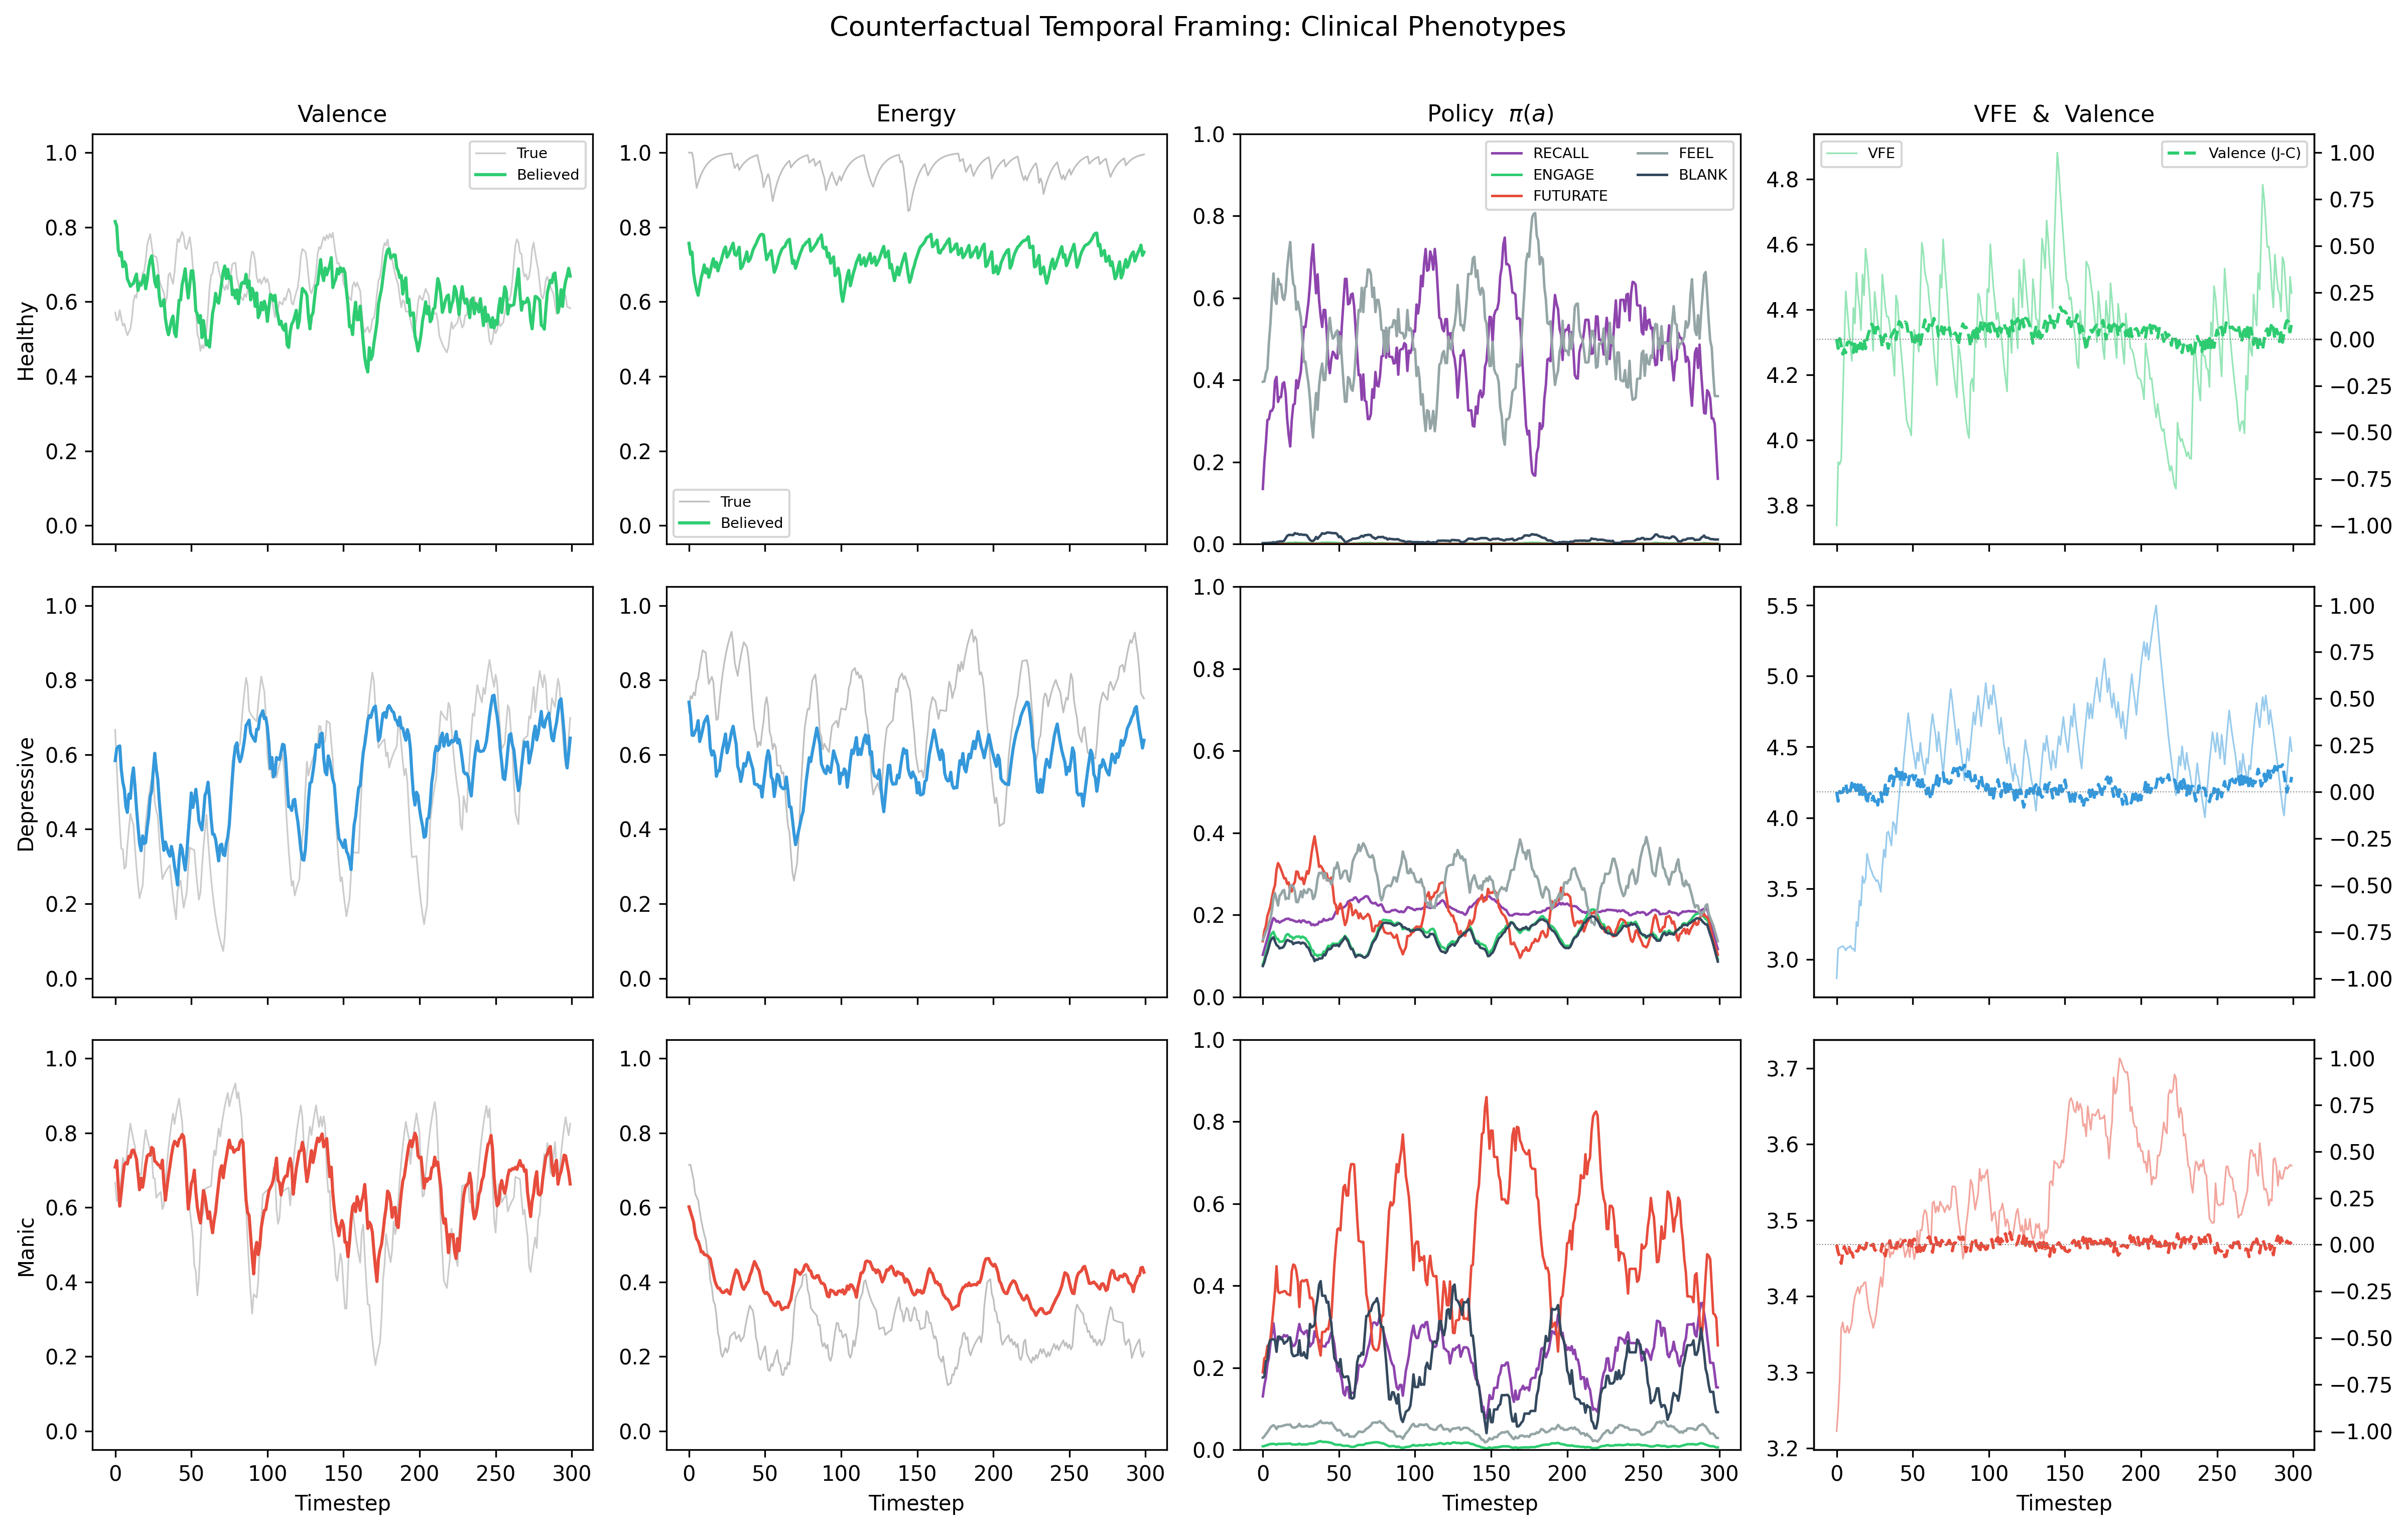
\includegraphics[width=\textwidth]{figures/fig1_phenotypes.png}
    \caption{\textbf{Phenotype comparison.} Each row corresponds to one clinical profile (healthy, depressive, manic). Columns show: (1) valence trajectories (true in gray, believed in colour, EMA-smoothed); (2) energy trajectories; (3) rolling policy probabilities $\pi(a)$ over a 15-step window; (4) variational free energy $F(t)$ (left axis) and Joffily-Coricelli valence $-\dot{F}$ (right axis, dashed). The healthy agent maintains high valence and near-maximal energy with RECALL-dominated policy. The depressive agent shows lower valence with near-uniform policy (anhedonia). The manic agent achieves the highest valence at the cost of energy depletion. $T = 300$, seed = 42.}
    \label{fig:phenotypes}
\end{figure}

\begin{figure}[t]
    \centering
    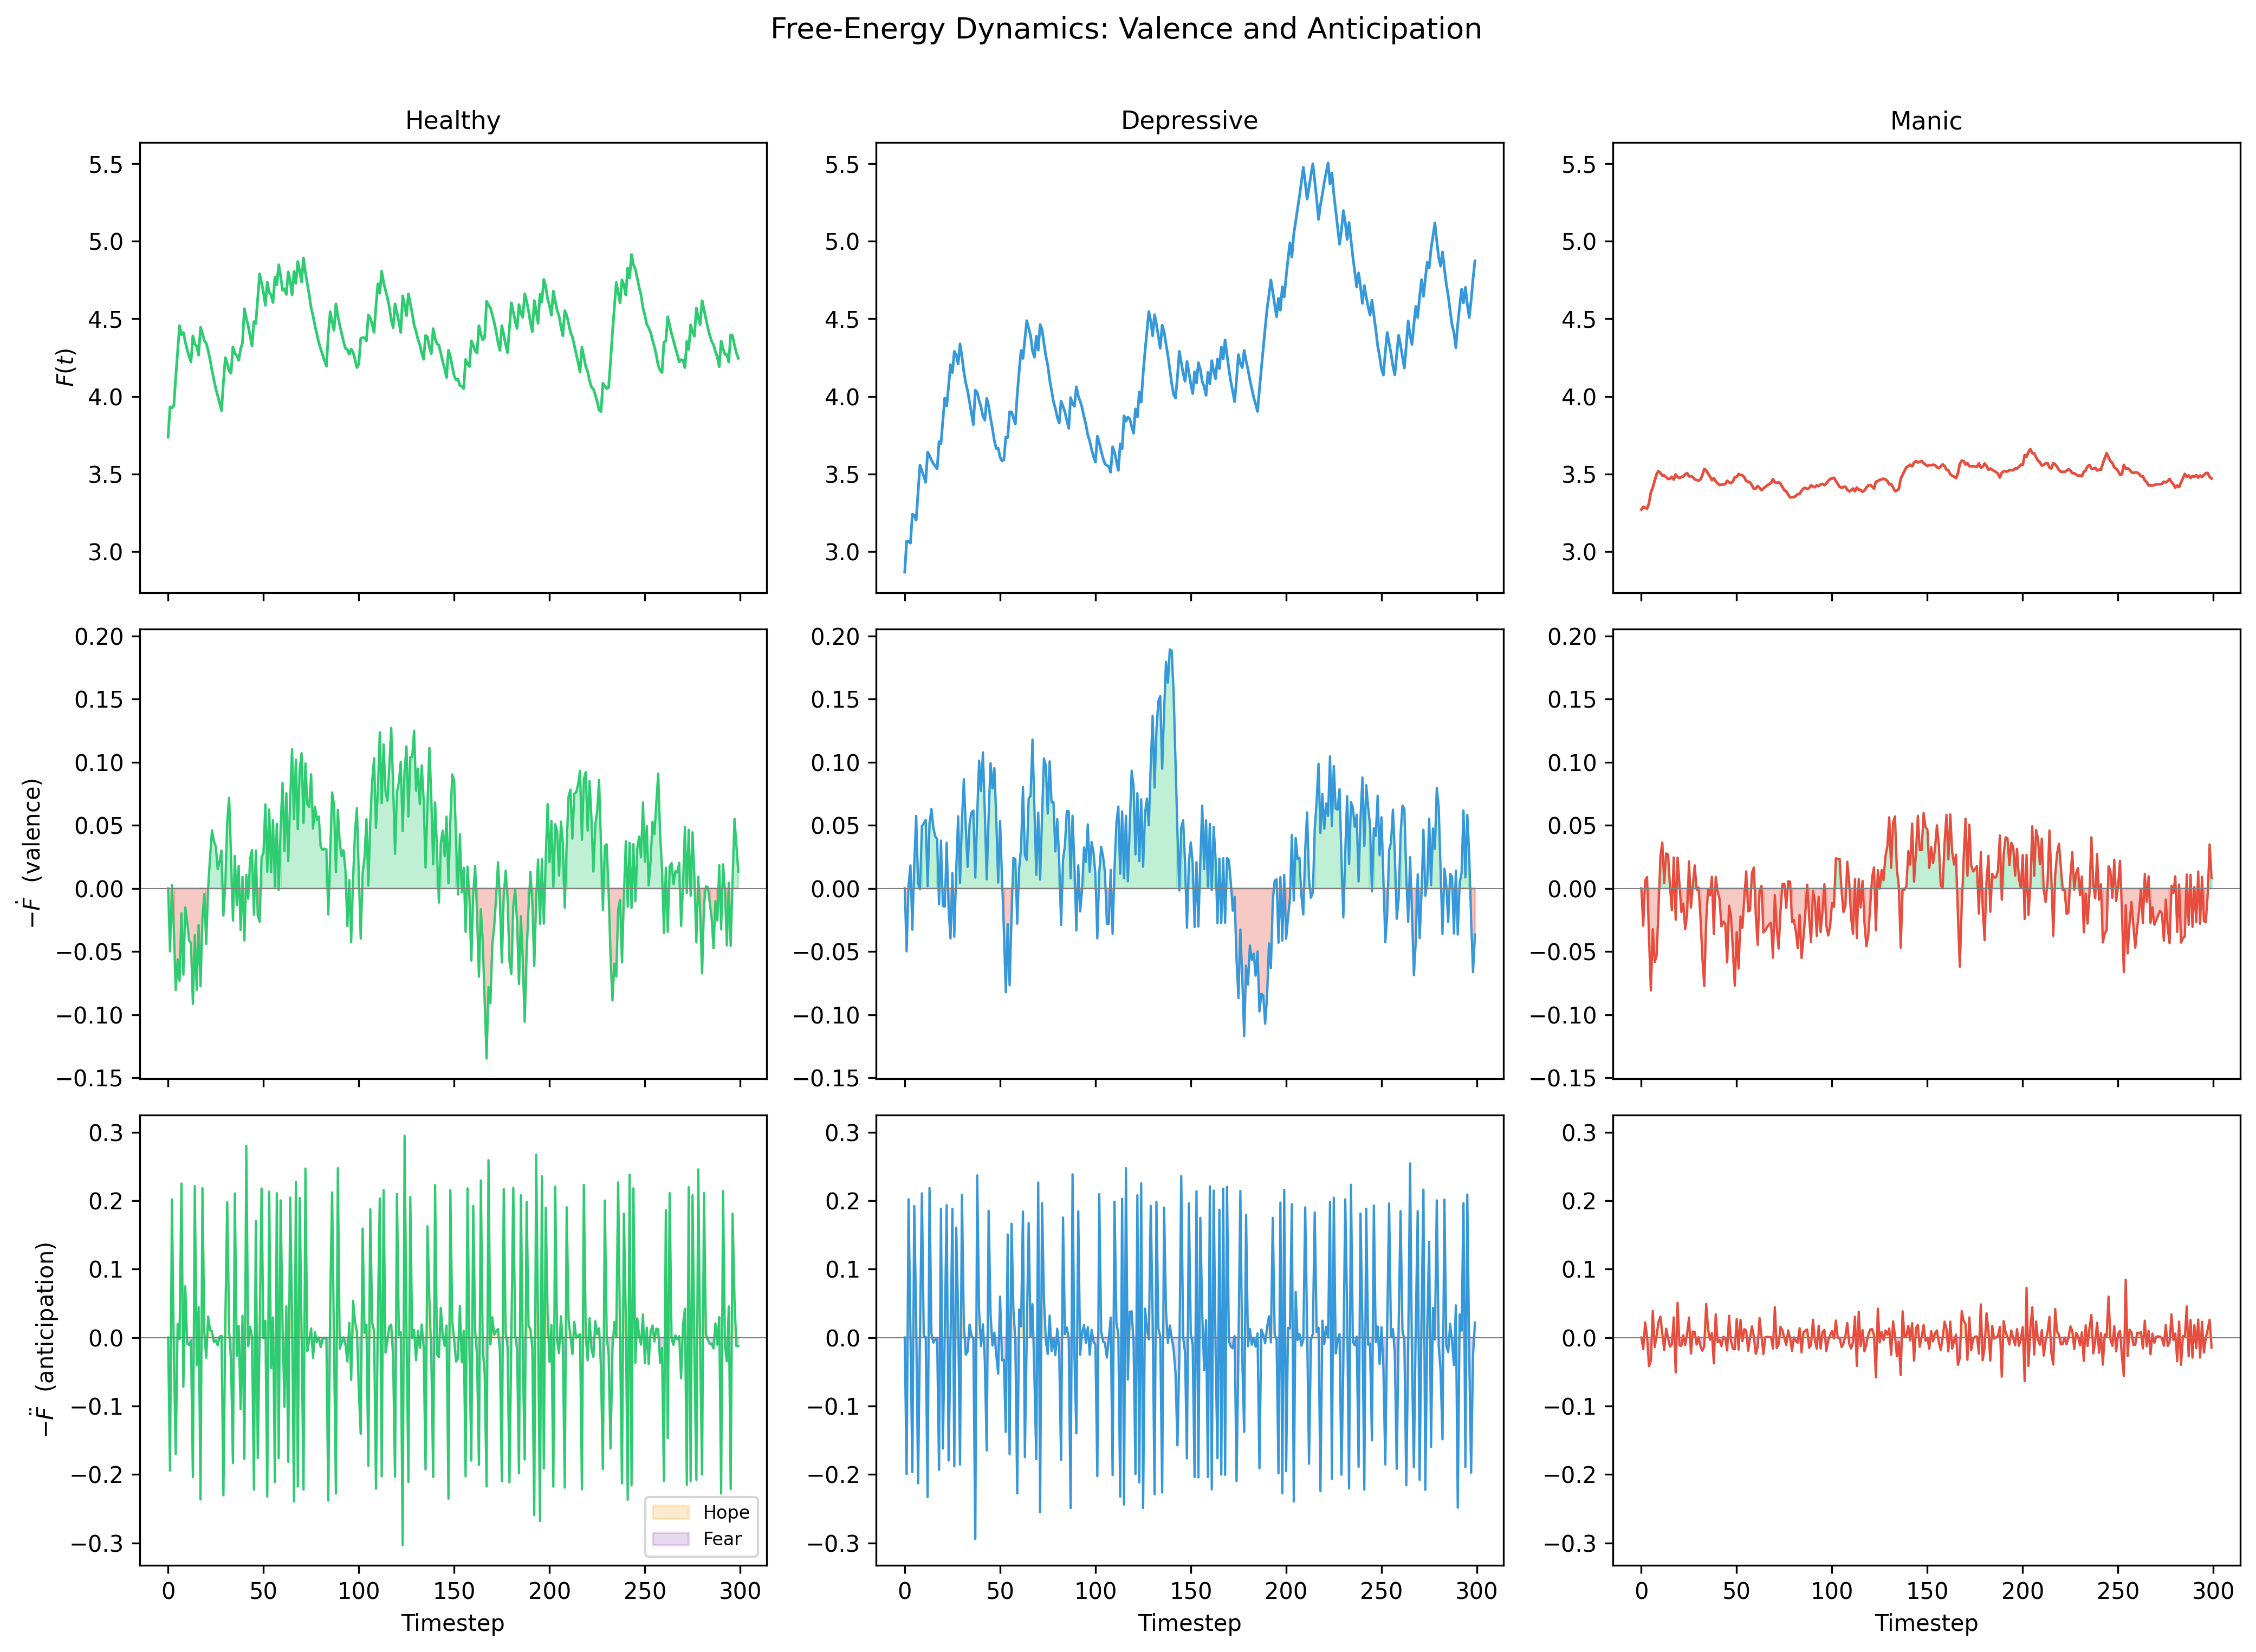
\includegraphics[width=\textwidth]{figures/fig2_joffily.png}
    \caption{\textbf{Free-energy dynamics} \citep{joffily2013emotional}. Columns correspond to phenotypes. Top: variational free energy $F(t)$. Middle: valence as $-\dot{F}$ (green = positive, red = negative). Bottom: anticipation as $-\ddot{F}$ (orange = hope, purple = fear). Y-axes are shared across columns within each row. The depressive agent shows rising $F(t)$ (worsening model fit); the manic agent's $F(t)$ is flat (overconfident model impervious to prediction errors).}
    \label{fig:joffily}
\end{figure}

\begin{figure}[t]
    \centering
    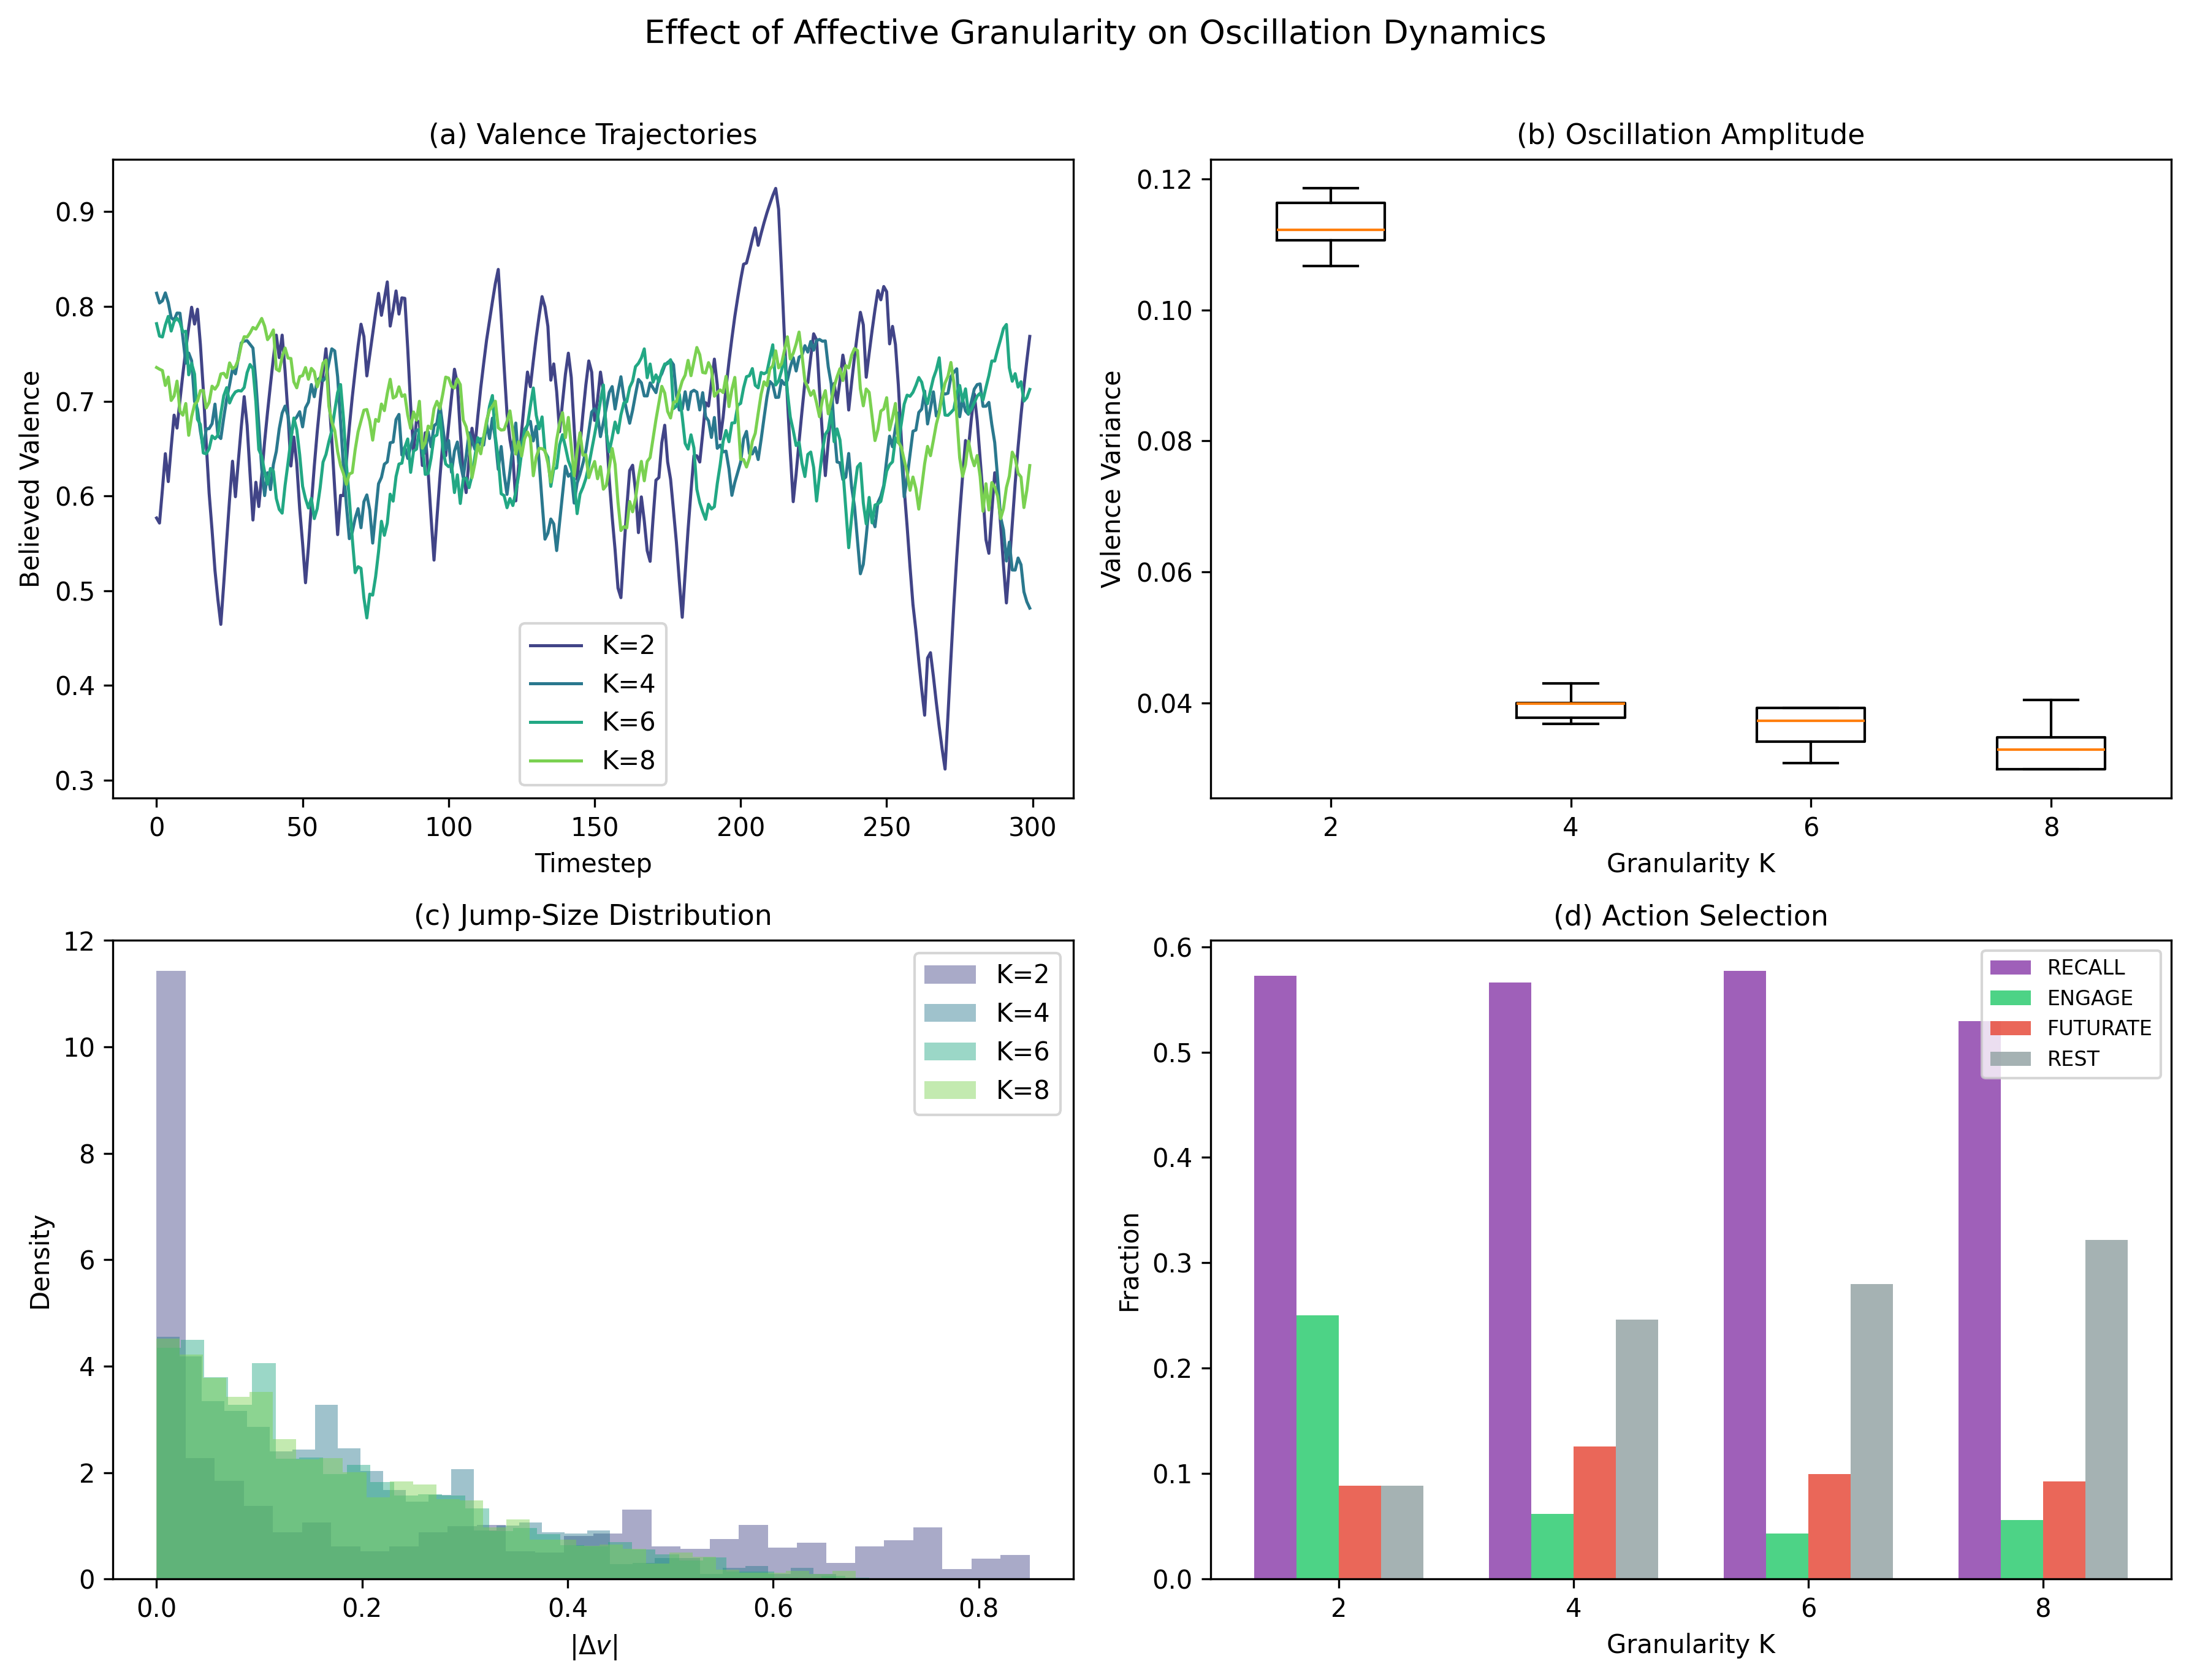
\includegraphics[width=\textwidth]{figures/fig3_granularity.png}
    \caption{\textbf{Effect of affective granularity on oscillation dynamics.} Fixed parameters: $\pi_{\text{pos}} = 3.0$, $\omega_e = 0.8$, $c_{\text{scale}} = 1.0$; $K \in \{2, 4, 6, 8\}$, 5 runs each. (a) Valence trajectories (EMA-smoothed). (b) Valence variance: $K{=}2$ shows substantially higher oscillation than $K \geq 4$. (c) Jump-size distribution: $K{=}2$ has a heavy tail (catastrophic transitions). (d) Action selection proportions: RECALL dominates across all $K$.}
    \label{fig:granularity}
\end{figure}

\begin{figure}[t]
    \centering
    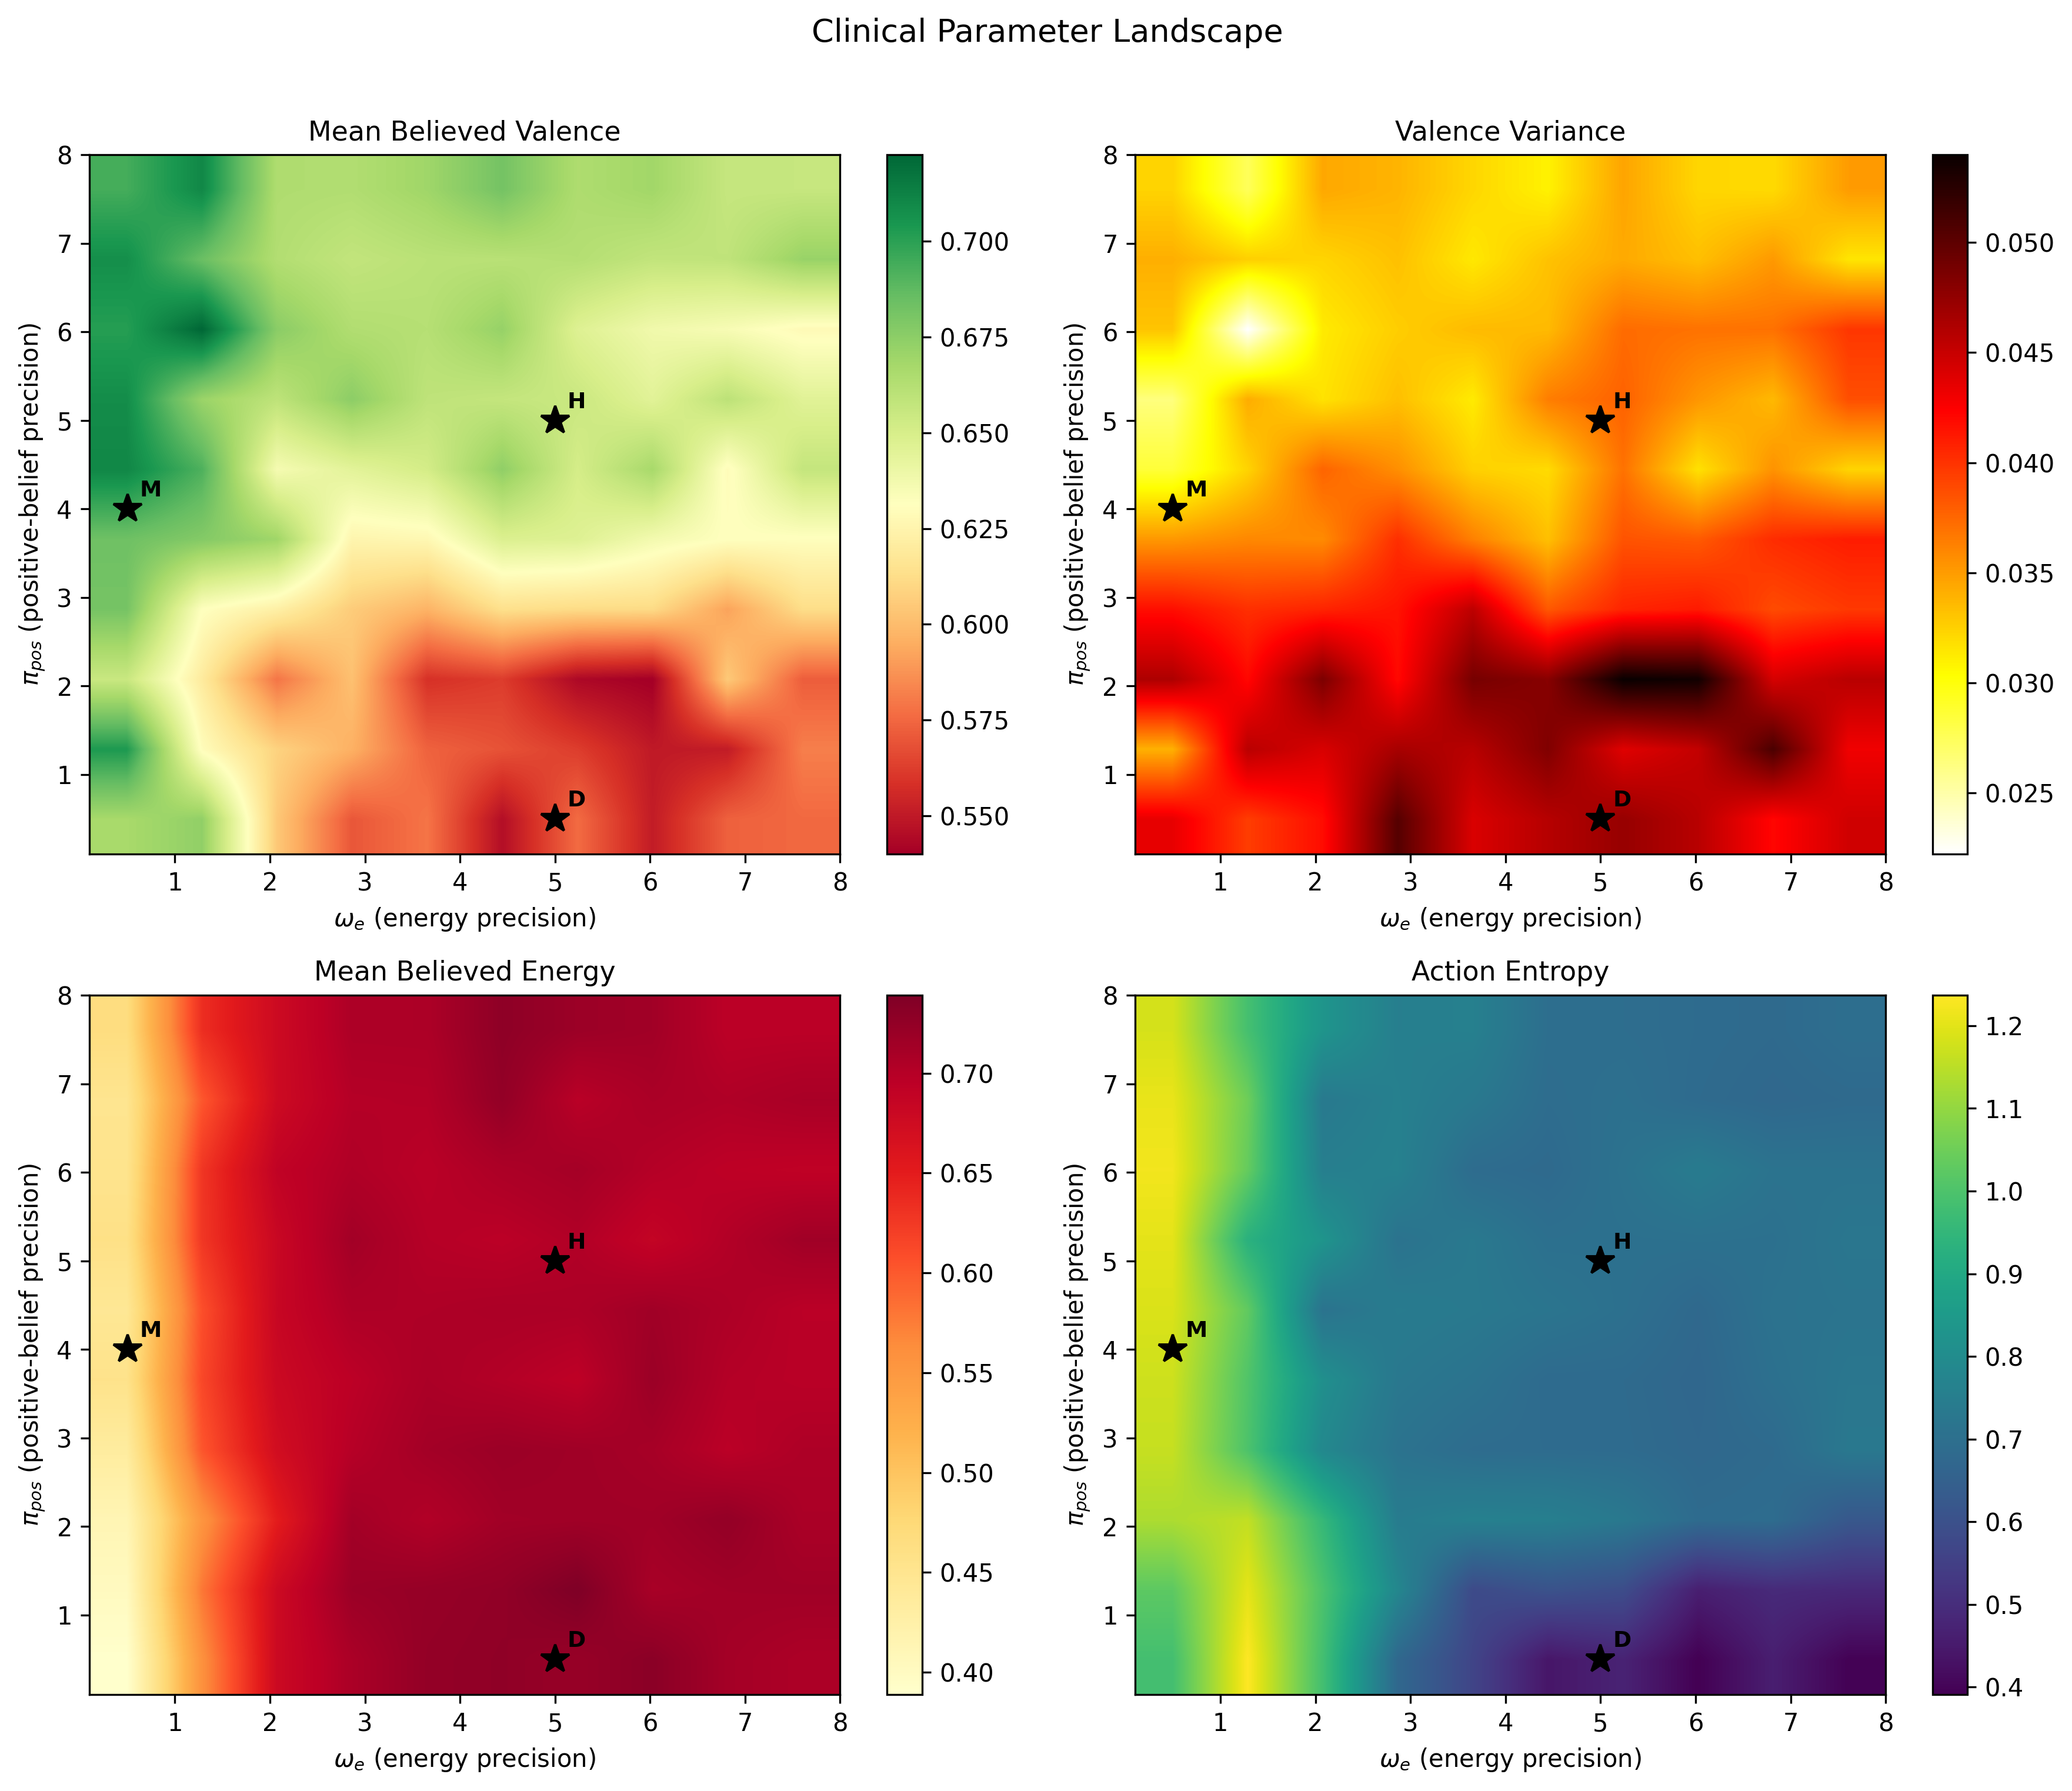
\includegraphics[width=\textwidth]{figures/fig4_parameter_space.png}
    \caption{\textbf{Clinical parameter landscape.} Heatmaps over $\pi_{\text{pos}} \times \omega_e$ (fixing $K{=}4$, $c_{\text{scale}} = 1.0$, $T{=}200$). Top left: mean believed valence. Top right: valence variance (peaks in the manic-vulnerable zone). Bottom left: mean believed energy (depleted at low $\omega_e$). Bottom right: action entropy (lowest at low $\pi_{\text{pos}}$). Stars: approximate phenotype locations (H = healthy, D = depressive, M = manic).}
    \label{fig:landscape}
\end{figure}

\begin{figure}[t]
    \centering
    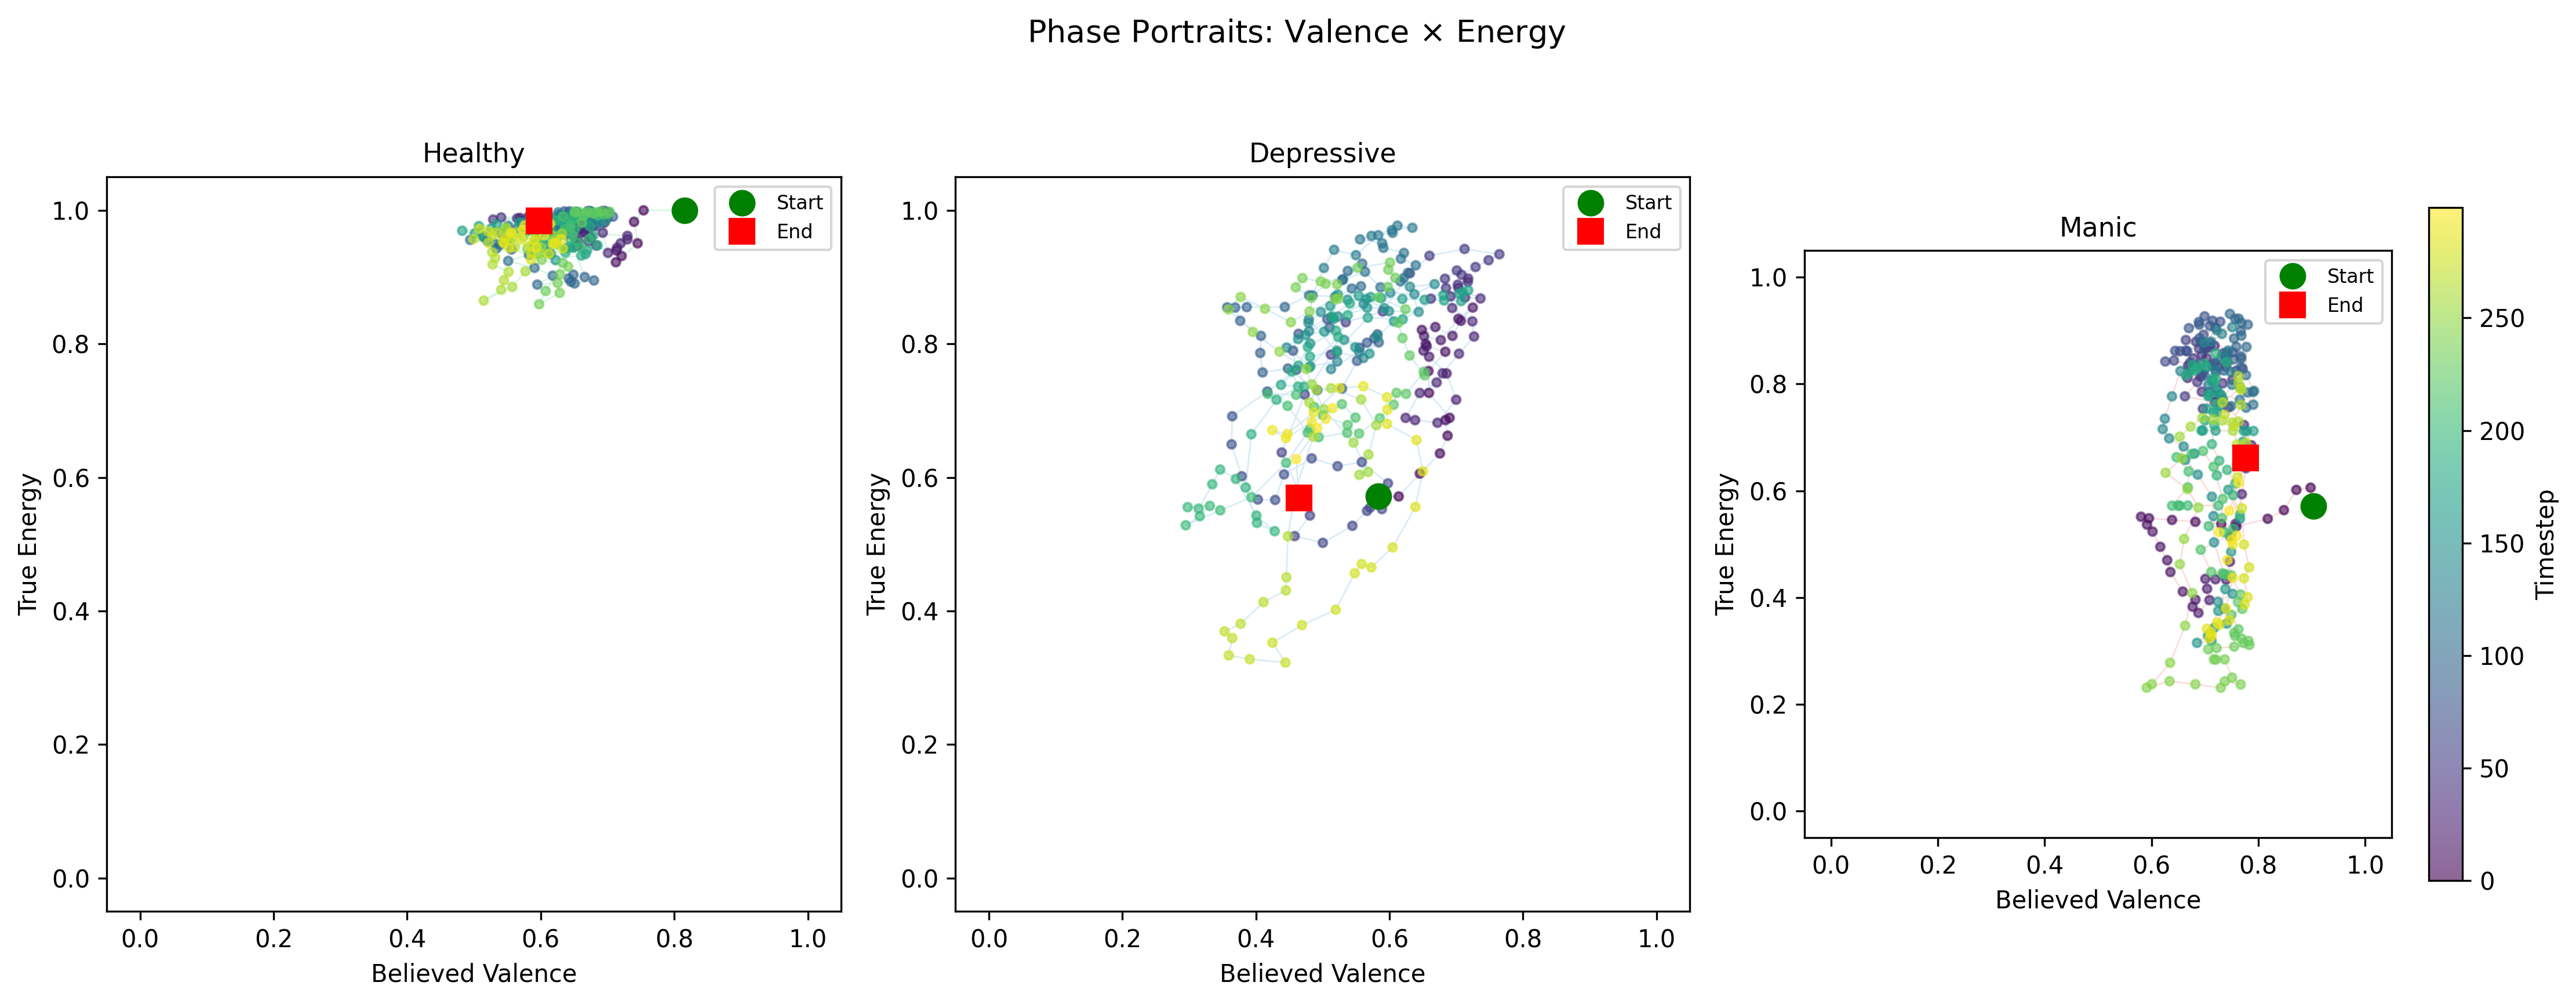
\includegraphics[width=\textwidth]{figures/fig5_phase_portrait.png}
    \caption{\textbf{Phase portraits: valence $\times$ energy.} EMA-smoothed believed valence vs.\ true energy; colour encodes timestep (purple = early, yellow = late). The healthy agent occupies a tight high-energy cluster (stable). The depressive agent wanders widely (emotional instability from near-random policy). The manic agent shows vertical energy spread---high valence across a wide energy range---reflecting the dissociation between subjective wellbeing and metabolic depletion.}
    \label{fig:phase}
\end{figure}

\begin{figure}[t]
    \centering
    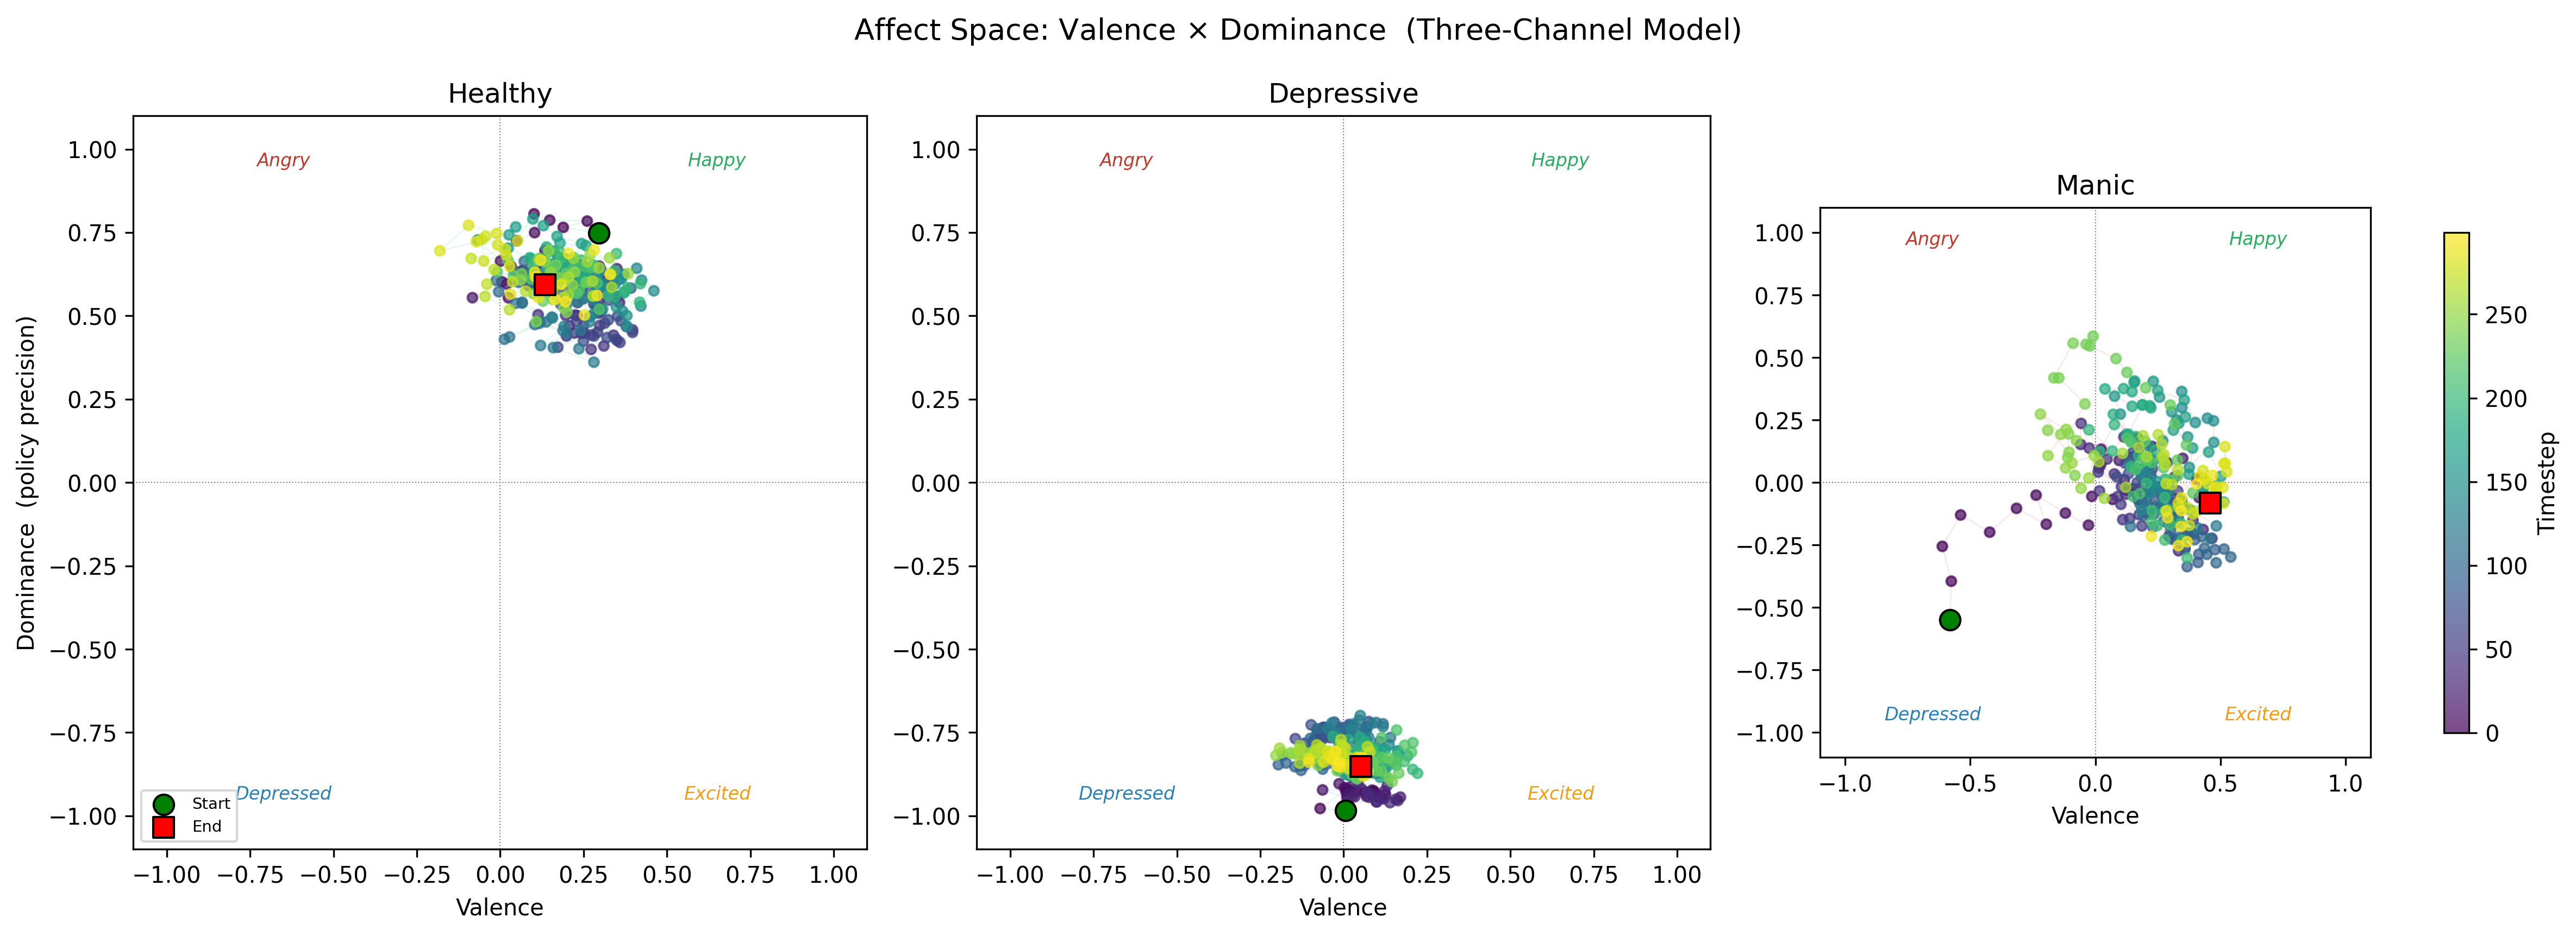
\includegraphics[width=\textwidth]{figures/fig6_circumplex.png}
    \caption{\textbf{Circumplex emotional trajectories} \citep{pattisapu2024free}. Polar plots of valence ($V = U - \mathbb{E}[U]$) and centred arousal ($A_c = 2H_{\text{norm}} - 1$). The healthy agent occupies a compact Happy/Excited region. The depressive agent shows the widest circumplex occupancy, extending into Angry and Sad quadrants (affect instability). The manic agent clusters tightly near Excited/Happy (elevated but narrow positive affect). R-limits shared across panels; colour encodes timestep.}
    \label{fig:circumplex}
\end{figure}
